\documentclass[a4paper,11pt]{article}%,twocolumn
%\documentclass[a4paper,11pt]{article}
%% packages

\usepackage{blindtext} % needed for creating dummy text passages
%\usepackage{ngerman} % needed for German default language
\usepackage{amsmath} % needed for command eqref
\usepackage{amssymb} % needed for math fonts
\usepackage[colorlinks=true,breaklinks]{hyperref} % needed for creating hyperlinks in the document, the option colorlinks=true gets rid of the awful boxes, breaklinks breaks lonkg links (list of figures), and ngerman sets everything for german as default hyperlinks language
\usepackage[hyphenbreaks]{breakurl} % ben�tigt f�r das Brechen von URLs in Literaturreferenzen, hyphenbreaks auch bei links, die �ber eine Seite gehen (mit hyphenation).
\usepackage{xcolor}
\definecolor{c1}{rgb}{0,0,1} % blue
\definecolor{c2}{rgb}{0,0.3,0.9} % light blue
\definecolor{c3}{rgb}{0.3,0,0.9} % red blue
\hypersetup{
    linkcolor={c1}, % internal links
    citecolor={c2}, % citations
    urlcolor={c3} % external links/urls
}
%\usepackage{cite} % needed for cite
\usepackage[square,authoryear]{natbib} % needed for cite and abbrvnat bibliography style
\usepackage[nottoc]{tocbibind} % needed for displaying bibliography and other in the table of contents
\usepackage{graphicx} % needed for \includegraphics 
\usepackage{longtable} % needed for long tables over pages
\usepackage{bigstrut} % needed for the command \bigstrut
\usepackage{enumerate} % needed for some options in enumerate
%\usepackage{todonotes} % needed for todos
\usepackage{makeidx} % needed for creating an index
\makeindex
\usepackage{gensymb}
\usepackage{url}
\usepackage{psfrag}
\usepackage{multirow}
\usepackage{subfigure}
%% page settings

\usepackage[top=20mm, bottom=20mm,left=25mm,right=25mm]{geometry} % needed for page border settings
\parindent=0mm % for space of first line of new text block
\sloppy % for writing with hyphenless justification (tries to)
\hyphenation{} % use hyphenation of tolerance parametershttp://www.jr-x.de/publikationen/latex/tipps/zeilenumbruch.html
\hyphenpenalty=10000
\exhyphenpenalty=10000
\usepackage{fancyhdr} % needed for head and foot options
%% my macros

%% Text fomats
\newcommand{\tbi}[1]{\textbf{\textit{#1}}}

%% Math fonts
\newcommand{\bbA}{\mathbb{A}}
\newcommand{\bbB}{\mathbb{B}}
\newcommand{\bbC}{\mathbb{C}}
\newcommand{\bbD}{\mathbb{D}}
\newcommand{\bbE}{\mathbb{E}}
\newcommand{\bbF}{\mathbb{F}}
\newcommand{\bbG}{\mathbb{G}}
\newcommand{\bbH}{\mathbb{H}}
\newcommand{\bbI}{\mathbb{I}}
\newcommand{\bbJ}{\mathbb{J}}
\newcommand{\bbK}{\mathbb{K}}
\newcommand{\bbL}{\mathbb{L}}
\newcommand{\bbM}{\mathbb{M}}
\newcommand{\bbN}{\mathbb{N}}
\newcommand{\bbO}{\mathbb{O}}
\newcommand{\bbP}{\mathbb{P}}
\newcommand{\bbQ}{\mathbb{Q}}
\newcommand{\bbR}{\mathbb{R}}
\newcommand{\bbS}{\mathbb{S}}
\newcommand{\bbT}{\mathbb{T}}
\newcommand{\bbU}{\mathbb{U}}
\newcommand{\bbV}{\mathbb{V}}
\newcommand{\bbW}{\mathbb{W}}
\newcommand{\bbX}{\mathbb{X}}
\newcommand{\bbY}{\mathbb{Y}}
\newcommand{\bbZ}{\mathbb{Z}}
\usepackage[ framed, numbered]{matlab-prettifier}%framed,%

\begin{document}

\begin{titlepage}
\center % Center everything on the page

%-------------------------------------------------------------------------------------
%	HEADING SECTIONS
%------------------------------------------------------------------------------------
\textbf{\large Department of Electronic and Telecommunication Engineering}\\[0.5cm]
\textbf{\Large University of Moratuwa, Sri Lanka}\\[1cm]
\textbf{\large EN 2053 - Communication Systems and Networks}\\[2cm]

\includegraphics[width=0.3\textwidth]{figures/uomlogo}\\[2cm]

	
%-------------------------------------------------------------------------------------
%	TITLE SECTION
%------------------------------------------------------------------------------------
\textbf{\Huge Modelling Propagation Losses and MANETs}\\[0.5cm]
\textbf{\Large Assignment 2}\\[5cm]


%----------------------------------------------------------------------------------------
%	MEMBERS SECTION
%----------------------------------------------------------------------------------------

\textbf{\large Submitted by}\\[0.5cm]
\begin{minipage}{0.2\textwidth}
	\begin{flushleft}
		{\large Thalagala B.P.}\\[4mm]
		{\large Sauranga H.W.C.}\\[4mm]
		
		
	\end{flushleft}
\end{minipage}
\hspace{5mm}
\begin{minipage}{0.2\textwidth}
	\begin{flushright}
		{\large 180631J }\\[4mm]
		{\large 180574K }\\[4mm]
		
	\end{flushright}
\end{minipage}\\[1.5cm]

%----------------------------------------------------------------------------------------
%	DATE SECTION
%----------------------------------------------------------------------------------------
\textbf{\large Submitted on}\\[0.5cm]
\textbf{\Large \today} % Date, change the \today to a set date if you want to be precise

%----------------------------------------------------------------------------------------

\vfill % Fill the rest of the page with whitespace

\end{titlepage}
\tableofcontents

\begin{center}
	\textbf{\textit{*PDF is clickable}}
\end{center}
\pagebreak
%%-----------------------------------------------------------------------
\section{Modeling the RF propagation Using Matlab}
%%-----------------------------------------------------------------------
\subsection{Relationship between Free Space Path Loss and Frequency}

\textit{Consider  following meanings for the parameters}\\

\begin{tabular}{l l }
	$P_{RX}$ & = Received Power at the Receiving Antenna\\
	$P_{TX}$ & = Transmitted Power at the Transmitting Antenna\\
	$f$ & = Frequency of the wave in Hz\\
	$f_{GHz}$ & = Frequency of the wave in GHz\\
	$d$& = Distance between the antennas in m\\
	$d_{km}$& = Distance between the antennas in km\\
	$G_{TX}$& = Directive gain of the Transmitter\\
	$G_{RX}$& = Directive gain of the Receiver\\
	$c$& = Velocity of the electromagnetic waves in a vacuum\\

\end{tabular}\\[1cm]


The relationship between above parameters can be given as follows
\[
\begin{split}
P_{RX} & = P_{TX}.\frac{c^2}{(4\pi.f.d)^2}.G_{TX}.G_{RX}
\end{split}
\]
From the above equation, free space path loss, say $L$
\[
\begin{split}
L = \frac{(4\pi.f.d)^2}{c^2}
\end{split}
\]

By considering $\ 10.log_{10}()$ in both sides, Free Space Path Loss in dB, say $L_{dB}$

\[
\begin{split}
10.\log_{10}(L) &= 10.\log_{10}(\frac{(4\pi.f.d)^2}{c^2})\\
L_{dB}& = 10.\log_{10}((4\pi.f.d)^2) - 10.\log_{10}(c^2)\\
&=20.\log_{10}(4\pi.f.d)-20.\log_{10}(c)\\
&=20.\log_{10}(4\pi)-20.\log_{10}(c) + 20.\log_{10}(f) + 20.\log_{10}(d)\\
&=20.\log_{10}(\frac{4\pi}{c}) + 20.\log_{10}(f) + 20.\log_{10}(d)\\
&= -147.5522168 + 20.\log_{10}(f_{GHz}.10^9) + 20.\log_{10}(d_{km}.10^3)\\
& = -147.5522168 + 20.\log_{10}(10^9)+ 20.\log_{10}(f_{GHz}) + 20.\log_{10}(10^3) + 20.\log_{10}(d_{km})\\
&= -147.5522168 + 180+ 20.\log_{10}(f_{GHz}) + 60 + 20.\log_{10}(d_{km})\\
&= -147.5522168 + 240+ 20.\log_{10}(f_{GHz}) + 20.\log_{10}(d_{km})\\
&= +92.44778322+20.\log_{10}(f_{GHz}) + 20.\log_{10}(d_{km})
\end{split}
\]
Since transmitter and receiver are located at distance of 10km apart, by substituting $d_{km}= 10$.\\

Free Space Path Loss in dB, $L_{dB}$ as a function of frequency in Giga Hertz

\[
\begin{split}
L_{dB}(f_{GHz})&=  +112.44778322+20.\log_{10}(f_{GHz})
\end{split}
\]

\textbf{\textit{Note : Axes of the following plots are given in the logarithmic scale and range of frequency was chosen from 50 GHz to 1000 GHz since some of the ITU-R models are only defined in the 10 GHz-1000 GHz range.}}

\begin{figure}[!h]
	\centering
	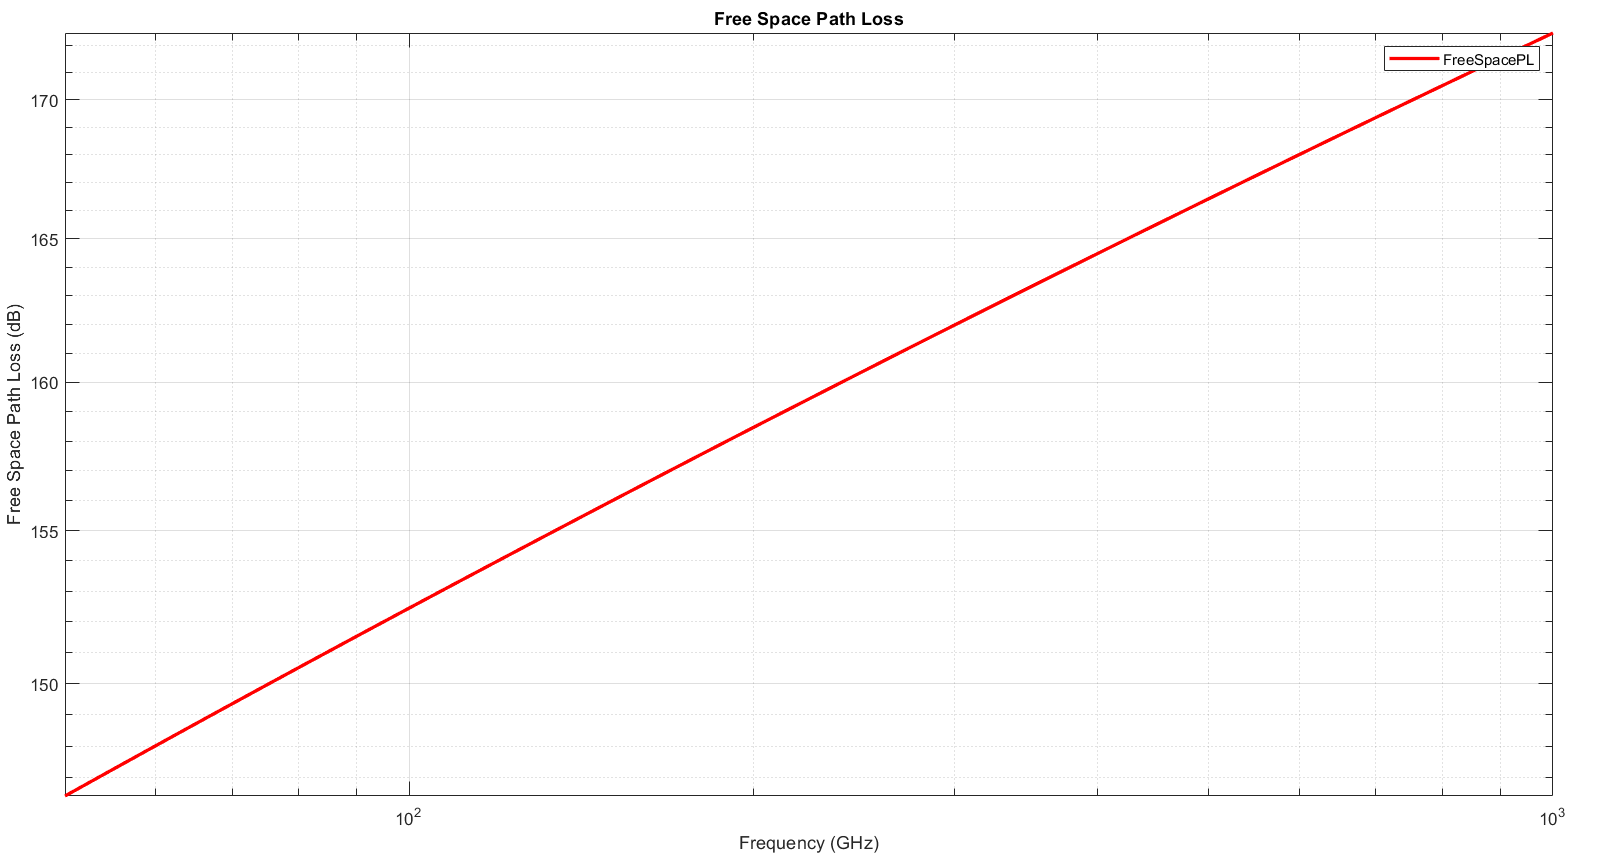
\includegraphics[scale=0.35]{figures/FreeSpacePL.png}
	\caption{Relationship between Free Space Path Loss and Frequency}
\end{figure}



%%-----------------------------------------------------------------------
\pagebreak
\subsection{Rain attenuation, Fog attenuation and Atmospheric gas attenuation with Frequency}

\textit{Note : For the generation of following plots three of the Matlab built-in functions, namely \textbf{rainpl()\cite{matlab}, gaspl()\cite{matlab}, fogpl()\cite{matlab}} which are developed according to the ITU-R P Series recommendations were used and links for their documentations are given at the Reference section.}


\subsubsection{Rain attenuation - Recommendation ITU-R P.838-3, 2005\cite{rain}}
The following plot shows how losses due to rain varies with frequency. The plot assumes the followings in addition to the provided information in the Task 1.\\

\begin{tabular}{l l}
Elevation angle of the propagation path& = 0 \\
Polarization tilt angle of the signal &= 0\\
\end{tabular}\\

In general, horizontal polarization represents the worse case for propagation loss due to rain.

\begin{figure}[!h]
	\centering
	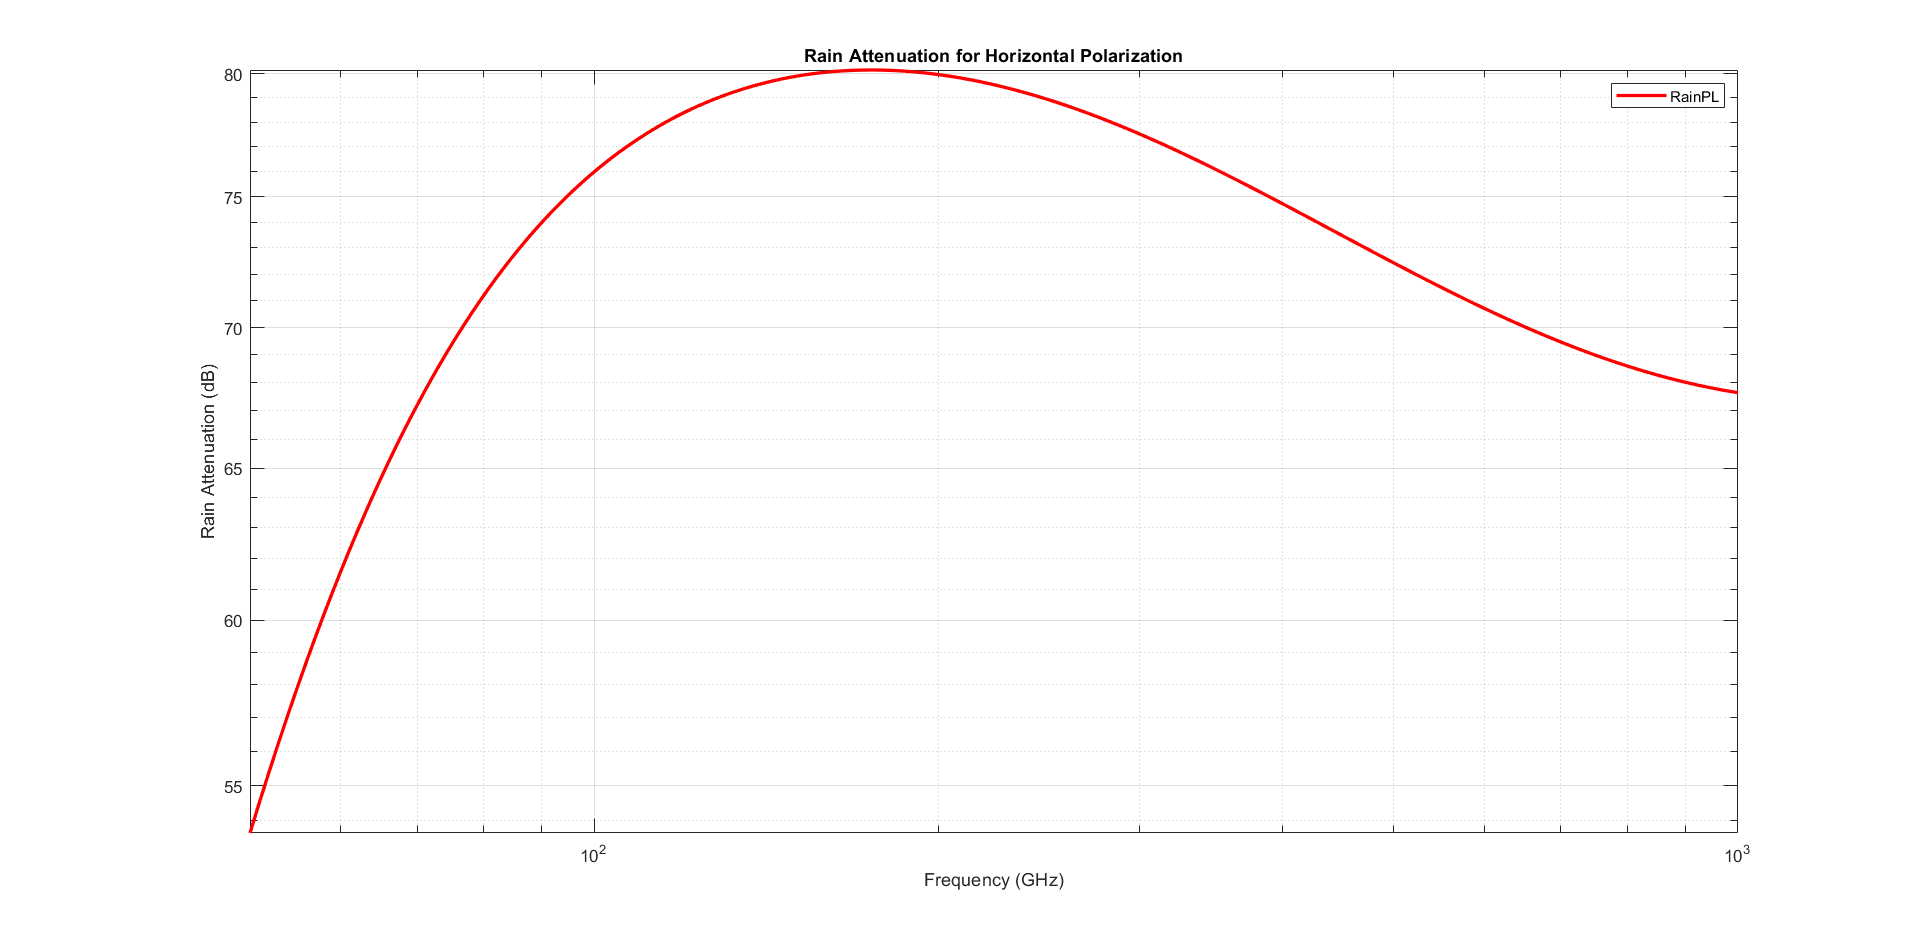
\includegraphics[scale=0.35]{figures/RainPL.png}
	\caption{Relationship between Rain attenuation and Frequency}
\end{figure}

\subsubsection{Fog attenuation - Recommendation ITU-R P.840-3, 2013\cite{fog}}
The following plot shows how losses due to fog/cloud varies with frequency. The plot assumes the following provided information in the Task 1.\\

\begin{tabular}{l l}
	Ambient Temperature in Celsius&= 31\\
	Liquid Water Density in $g/m^3$&= 0.5\\
\end{tabular}\\

\begin{figure}[!h]
	\centering
	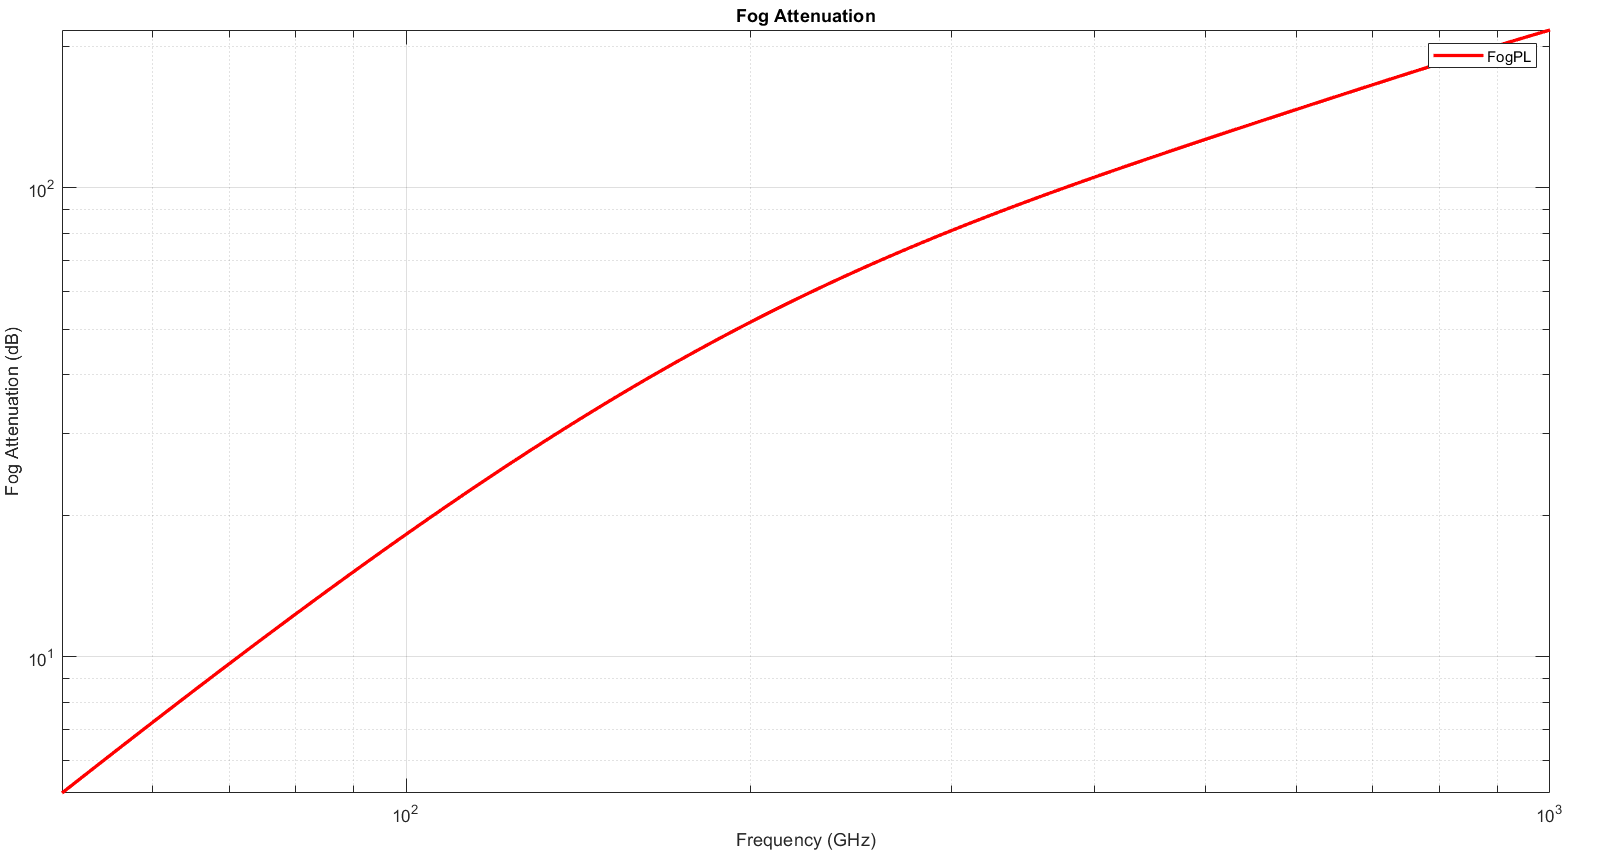
\includegraphics[scale=0.35]{figures/FogPL.png}
	\caption{Relationship between Fog attenuation  and Frequency}
\end{figure}

\subsubsection{Atmospheric gas attenuation - Recommendation ITU-R P.676-10, 2013\cite{gas}}

The plot below shows how the propagation loss due to atmospheric gases varies with the frequency. The plot assumes the followings in addition to the provided information in the Task 1.

\begin{tabular}{l l}
	 Dry air pressure in Pa&= 101325\\
	 Water Vapor Density in $g/m^3$&= 30.4\cite{vapor}\\
\end{tabular}


\begin{figure}[!h]
	\centering
	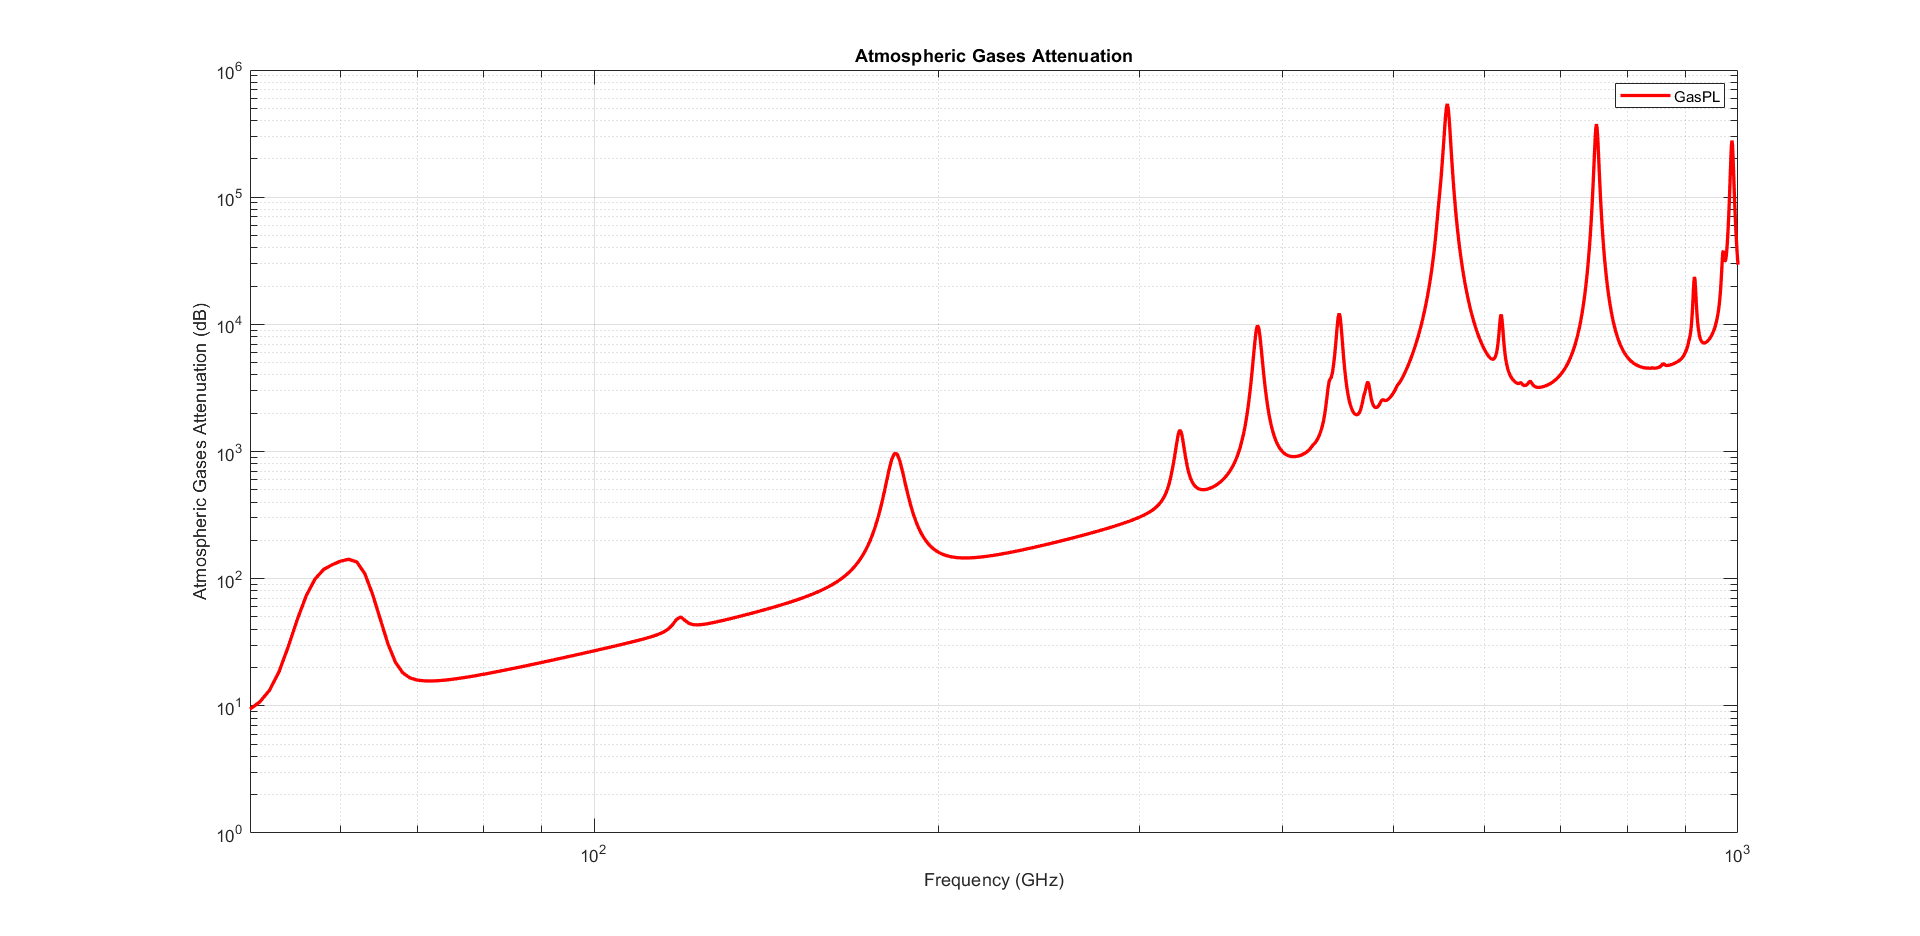
\includegraphics[scale=0.35]{figures/GasPL.png}
	\caption{Relationship between Atmospheric gas attenuation and Frequency}
\end{figure}


%%-----------------------------------------------------------------------
\subsection{Total Path Loss with Frequency}
\textit{Note : Range of frequency was chosen from 50 GHz to 1000 GHz since some of the ITU-R models are only defined in 10 GHz - 1000 GHz range.}
\begin{figure}[!h]
	\centering
	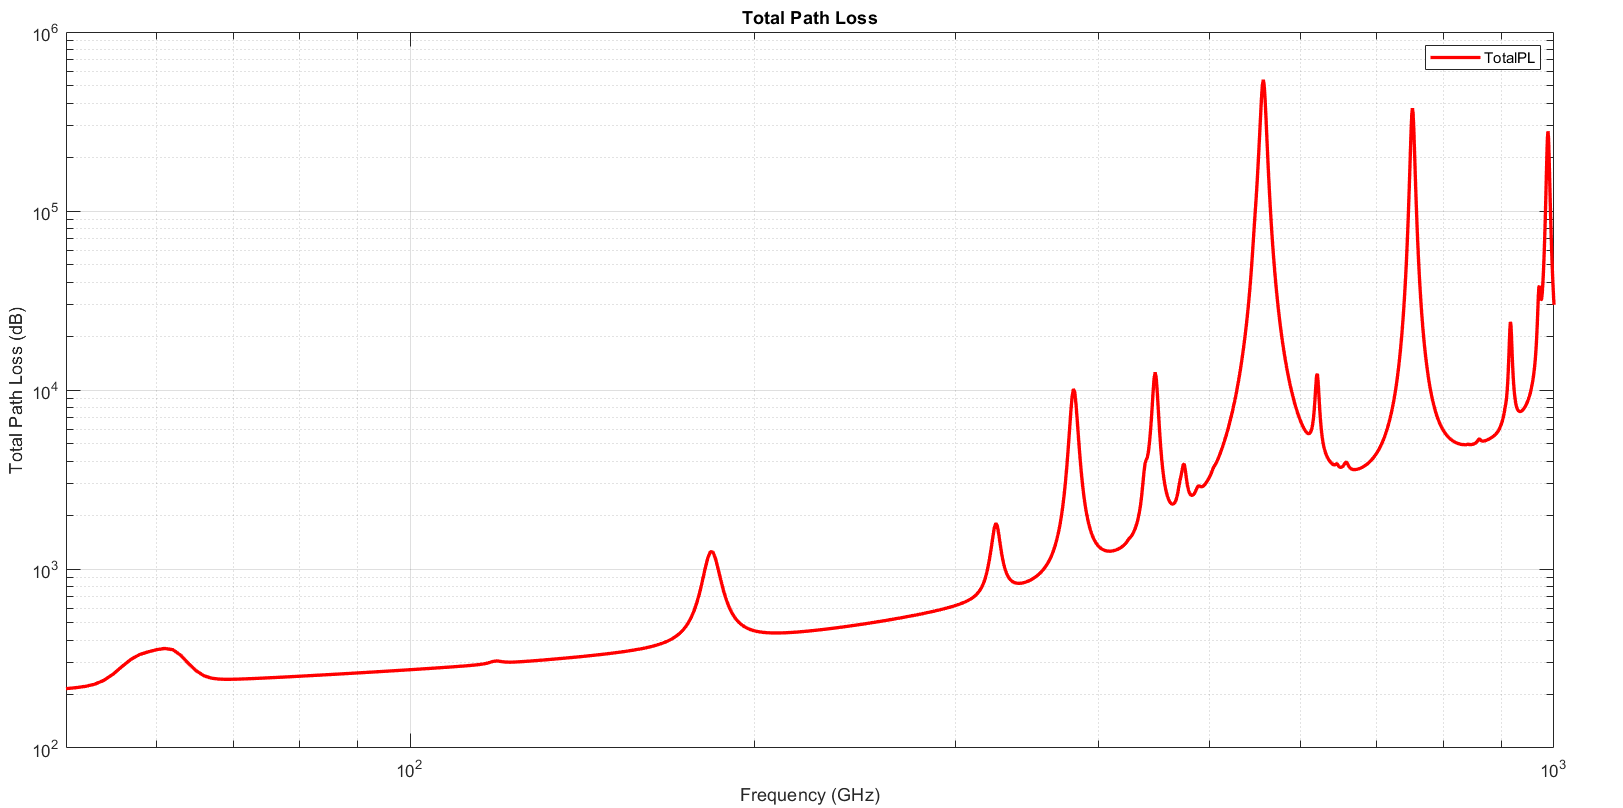
\includegraphics[scale=0.35]{figures/TotalPL.png}
	\caption{Relationship between Total Path Loss and Frequency}
\end{figure}

By inspecting the figure we can conclude that the minimum propagation loss is given at the frequency of 50 GHz in the given range. Therefore from this point onward, for the calculations it will be the frequency for transmission.\\

Minimum Propagation Loss = 214.624 dB\\
Corresponding Frequency = 50 GHz\\



\begin{figure}[!h]
	\centering
	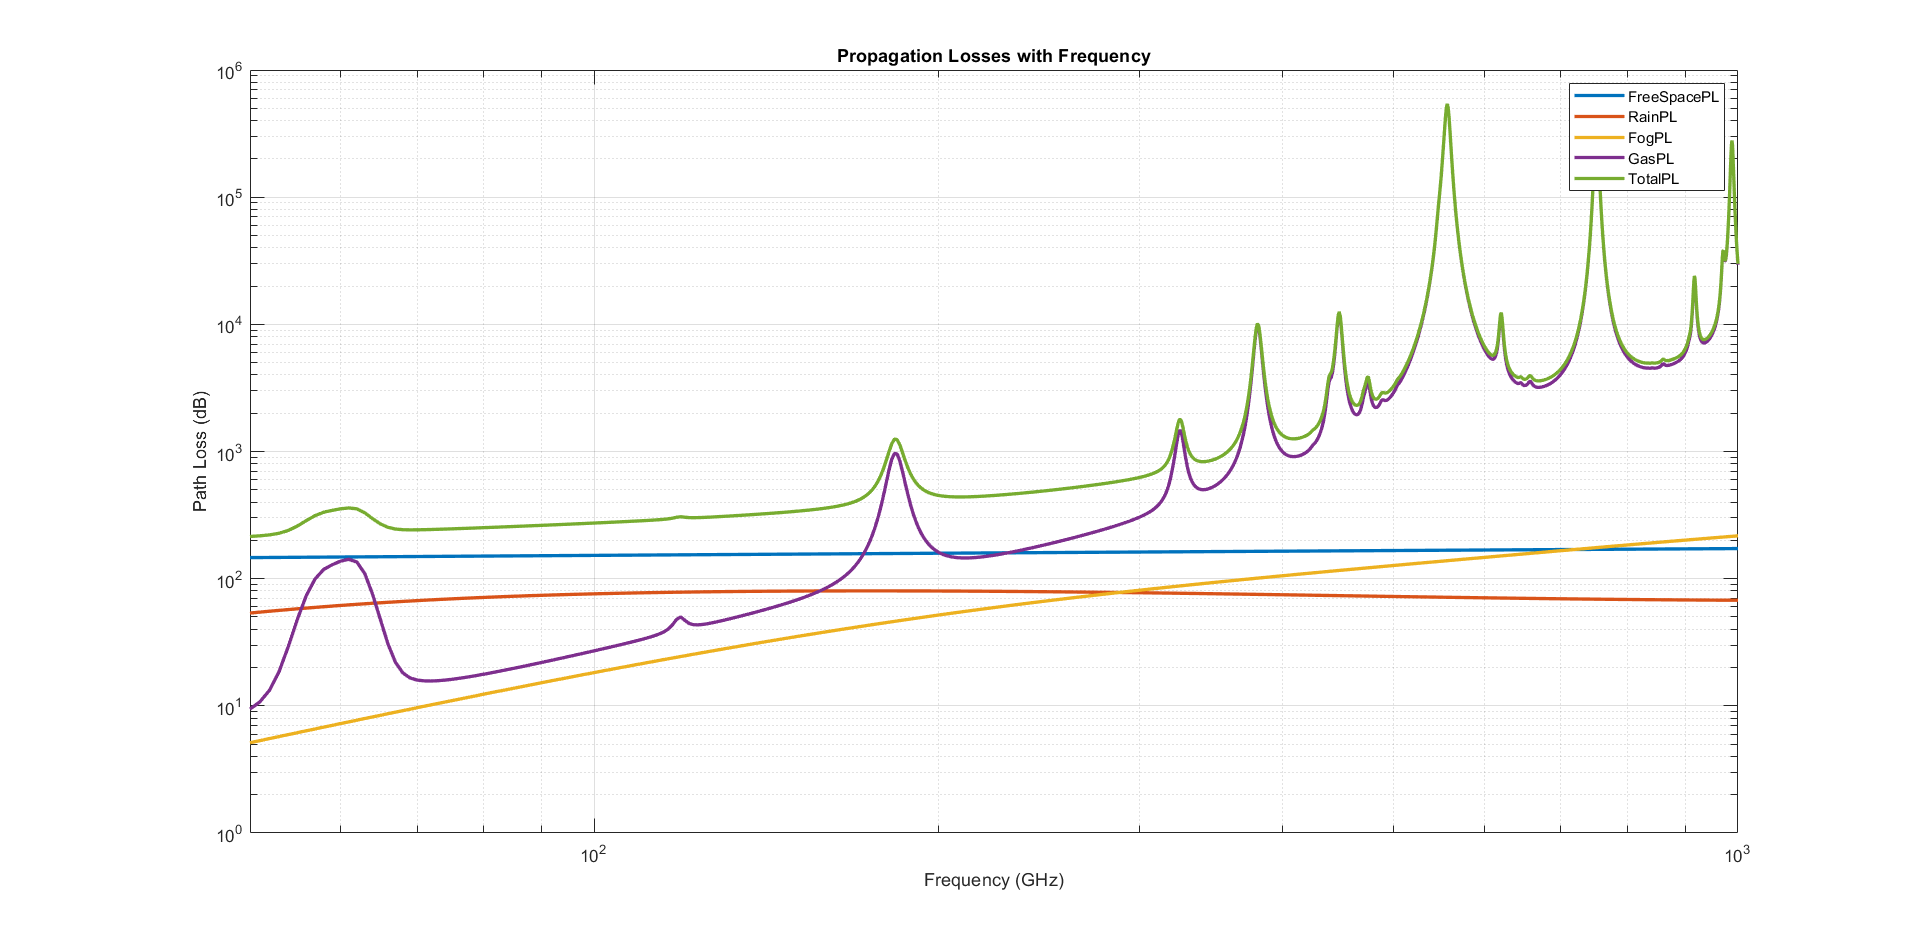
\includegraphics[scale=0.35]{figures/AllinOne.png}
	\caption{Relationship between Various Path Losses and Frequency - All in One}
\end{figure}
%\subsection{Link Budget Calculation}
%
%Parameters For the propagation model
%\begin{tabular}{l r}
%Chosen transmission frequency & 10 GHz\\
%Total Path Loss & 136.9 dB\\
%Transmission power & 50 kW or 47 dB\\
%Transmitter Gain & 30 dB\\
%Receiver Gain &24.77 dB\\
%Link margin  &11 dB\\
%Cable loss at Transmitter & 3 dB\\
%Cable loss at Receiver &4 dB\\
%\end{tabular}\\[1cm]
%
%Let's find the actual received power at the receiver\\
%
%\begin{tabular}{|l l| r|}
%	\hline
%Received Power =	&Transmission power & +47 dB\\
%&	Cable loss at Transmitter & -3 dB\\
%&	Transmitter Gain & 30 dB\\
%&	Total Path Loss & -136.9 dB\\
%&	Receiver Gain &+24.77 dB\\
%&	Cable loss at Receiver &-4 dB\\\hline
%Received Power =&&-42.13 dB\\\hline\hline
%\end{tabular}\\[1cm]
%
%
%Therefore,\\
%\begin{center}
%	\begin{tabular}{l c c c}
%Link margin  & =& Received Power& - Receiver Sensitivity\\
%11 dB& = &-42.13 dB& - Receiver Sensitivity\\
%Receiver Sensitivity &= &-53.13 dB& \\\hline\hline
%	\end{tabular}
%\end{center}

\pagebreak
\subsection{Variation of the Signal Power with the Distance}

Parameters For the propagation model\\

\begin{tabular}{l r}
Chosen Carrier frequency & 50 GHz\\
Transmission power & 50 kW or 47 dB\\
Cable loss at Transmitter & 3 dB\\
Transmitter Gain & 30 dB\\
Receiver Gain &24.77 dB\\
Cable loss at Receiver &4 dB\\
Total Path Loss & Varies with Distance\\
\end{tabular}\\[1cm]

According to above values, Let's calculate the Power of the signal when leaving the  Transmission antenna, say $P_{dB}(0~km)$,

\[
\begin{split}
P_{dB}(0~km) & = Transmission~power -  Cable~loss~at~Transmitter + Transmitter~Gain\\
&=47-3+30\\
&=74~dB
\end{split}
\]

Free Space Path Loss in dB, $L_{dB}$ as a function of distance in kilo meters. By substituting $f_{GHz}$ = 50 to the equation derived in part 1.

\[
\begin{split}
L_{dB}(d_{km})&= +92.44778322+20.\log_{10}(50) + 20.\log_{10}(d_{km})\\
&=+92.44778322+ 33.97940009 + 20.\log_{10}(d_{km})\\
&=+126.4271833+ 20.\log_{10}(d_{km})\\
\end{split}
\]

Therefore, \[Total~Path~Loss = L_{dB}(d_{km}) + Rain~Attenuation+Fog~Attenuation+Atmospheric~Gas~Attenuation \]

Therefore the Signal Power when reaching the Receiving Antenna at $d_{km}$ distance,
\[
\begin{split}
P_{dB}(d_{km}) & =74~dB - Total~Path~Loss
\end{split}
\]

\begin{figure}[!h]
	\centering
	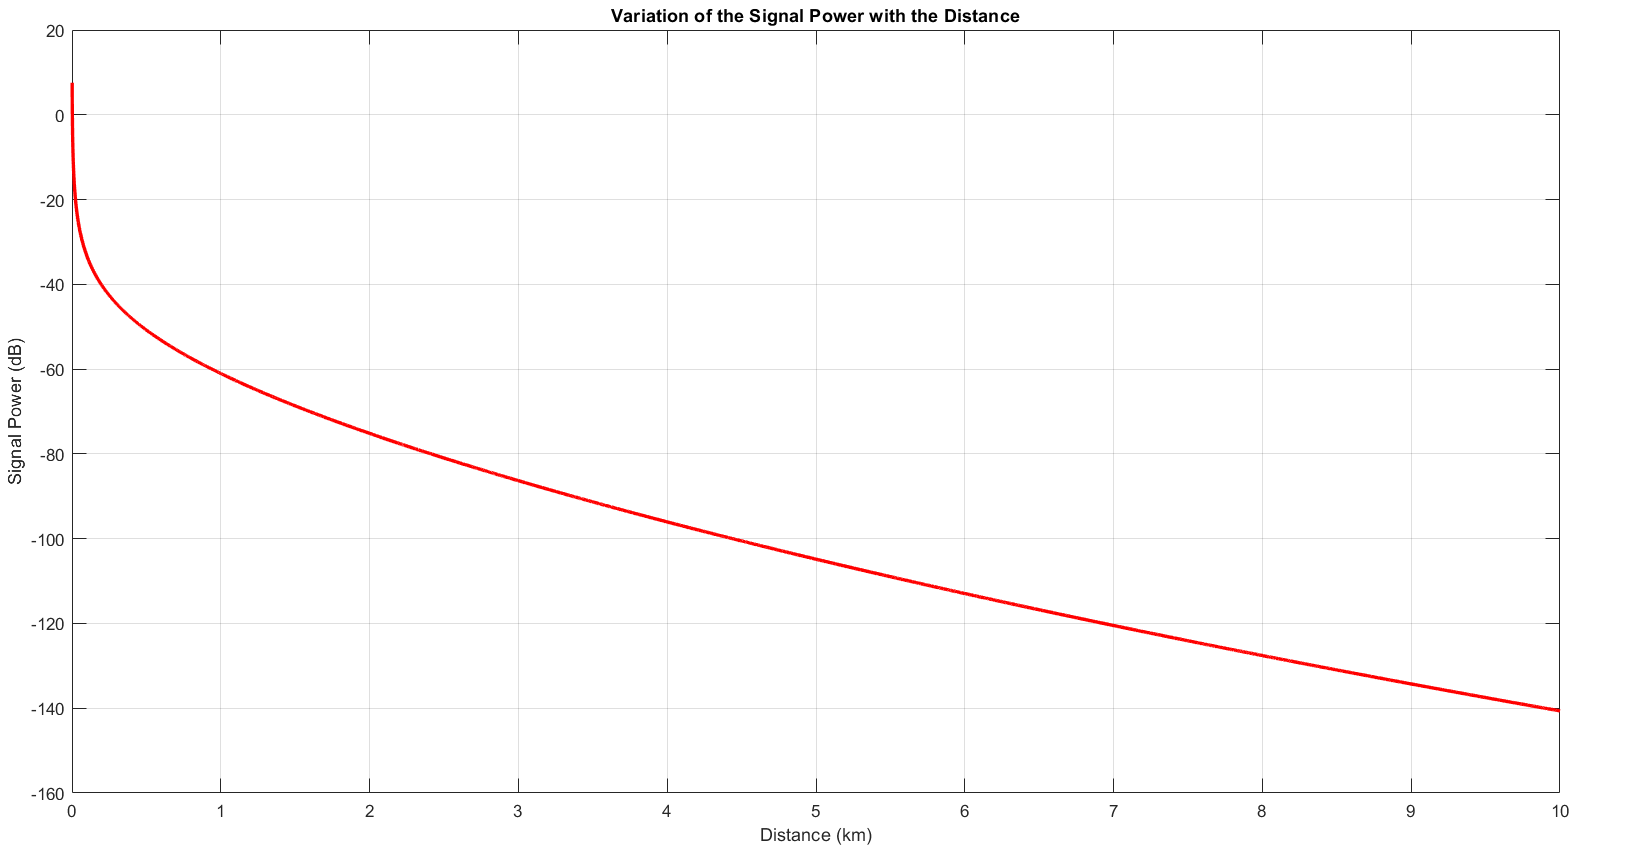
\includegraphics[scale=0.35]{figures/sp}
	\caption{Variation of the Signal Power with the Distance}
\end{figure}
\pagebreak

\subsection{Transmitting a voice signal over a noisy channel using the above Transmission frequency and the Propagation model.}

\begin{figure}[!h]
	\centering
	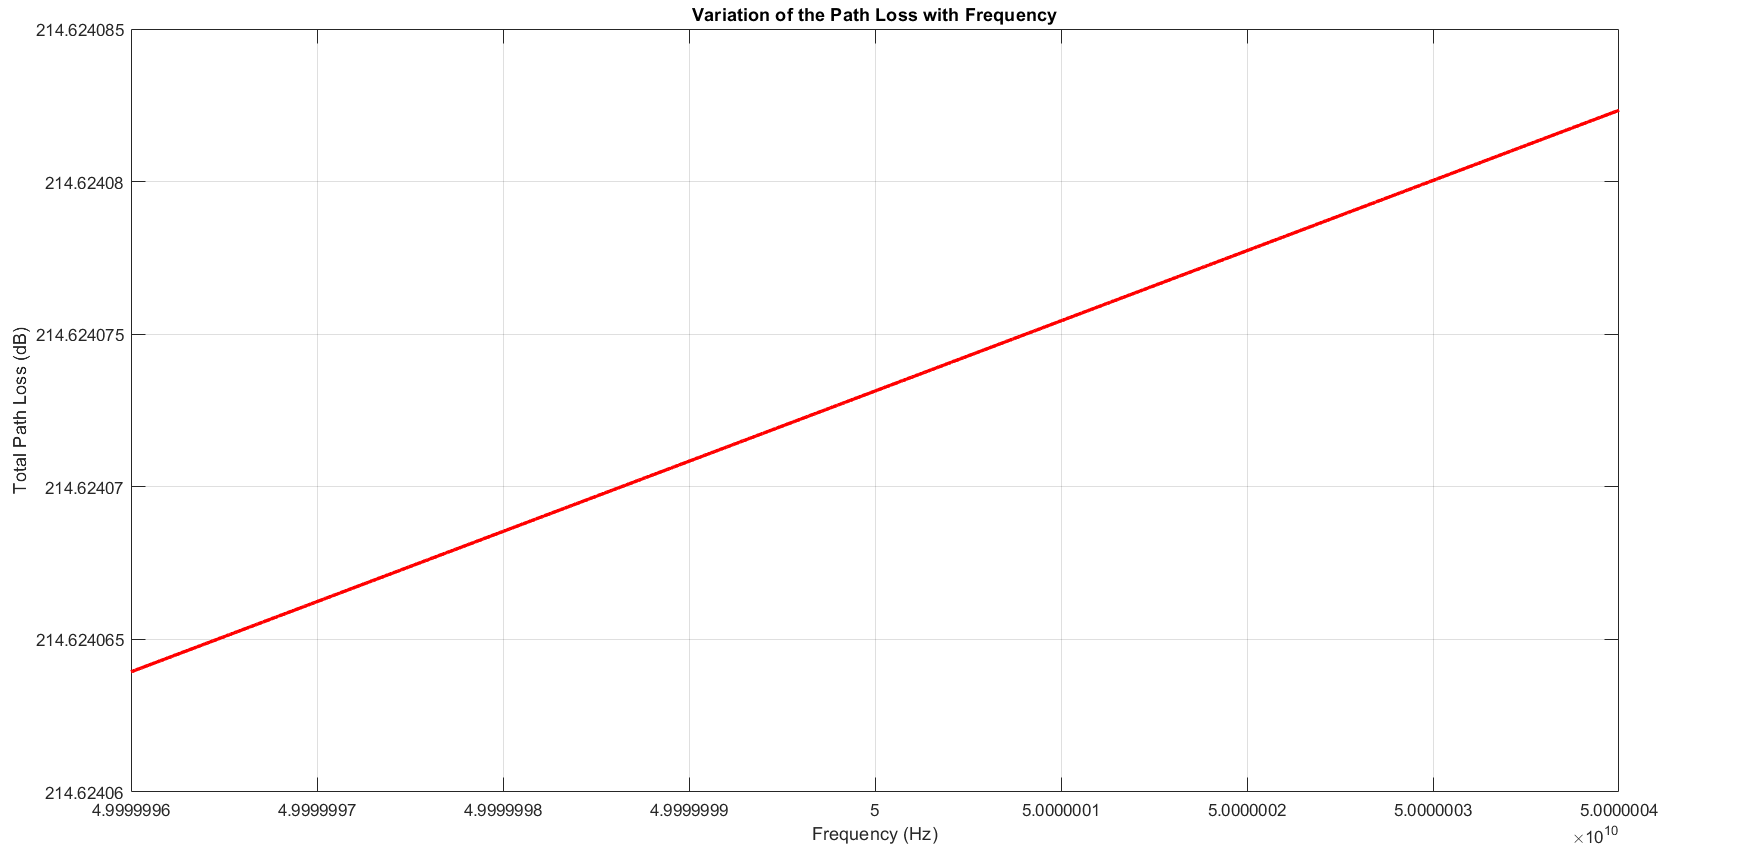
\includegraphics[scale = 0.36]{figures/voicePL}
	\caption{Variation of the Path Loss with Frequency in the Voice Signal}
\end{figure}

By inspecting the above figure, it can be concluded that the total Path Loss of the modulated Voice Signal is almost the same as that of the carrier wave (50 GHz) and therefore path loss variation due to the frequency in the above range can be neglected and can be assumed as a constant of 214.6240 dB.\\ 
Therefore for the following model, total path loss of the signal was taken as 214.6240 dB and it is included in the Free Space Loss block.

\subsubsection{RF Propagation Model - Simulink}

\begin{figure}[!h]
	\centering
	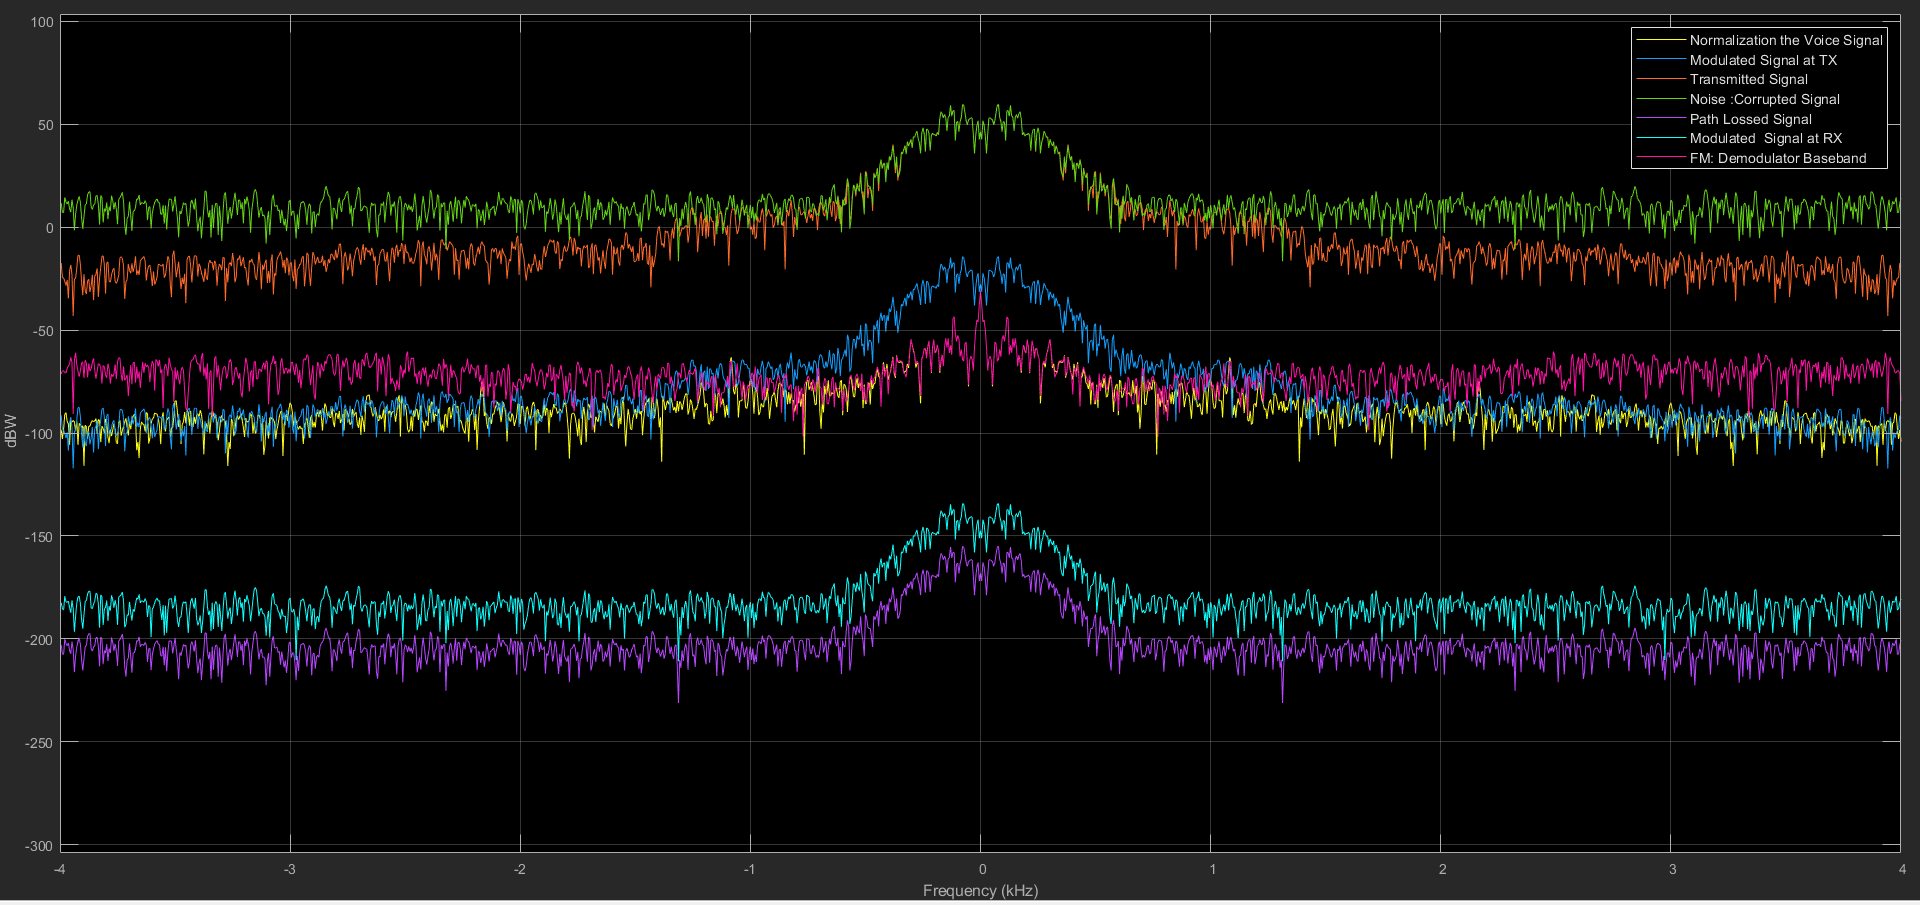
\includegraphics[scale = 0.42]{figures/spect2}
	\caption{Frequency Spectrum of the signal at Various States}
\end{figure}

\begin{figure}[!h]
	\centering
	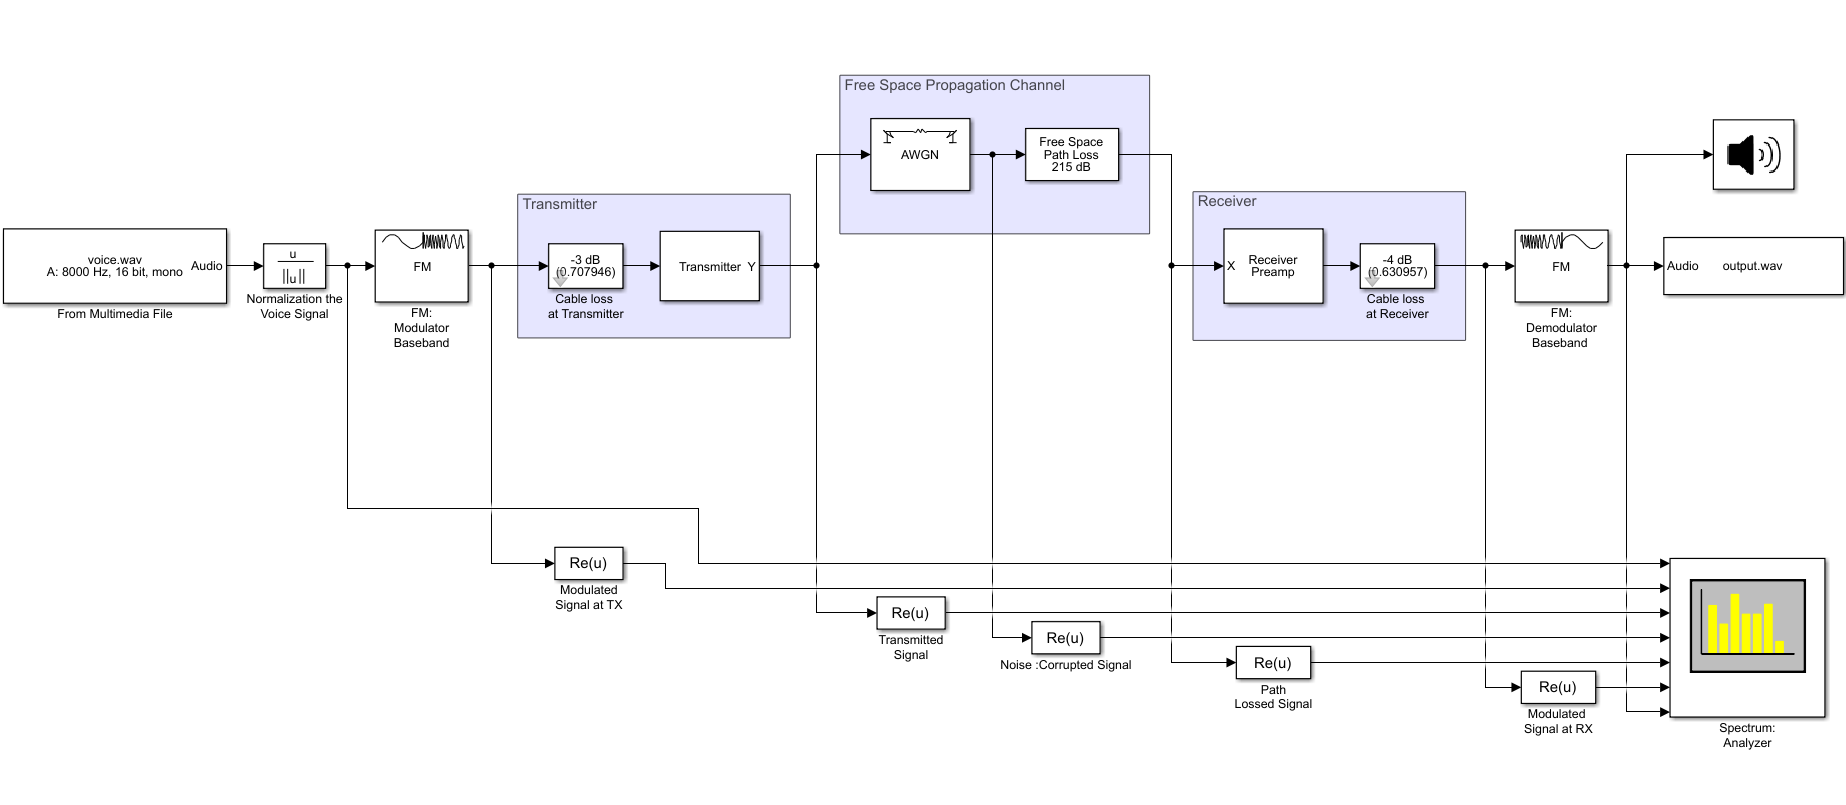
\includegraphics[scale = 0.64, angle= 90]{figures/model}
	\caption{RF Propagation Model - Simulink}
\end{figure}


\pagebreak
\subsection{Codes for Task 1}
\lstinputlisting[basicstyle = \mlttfamily\scriptsize , style = Matlab-editor]{code/RFPL.m}

\lstinputlisting[basicstyle = \mlttfamily\scriptsize , style = 
Matlab-editor]{code/plotCurve.m}
\vfill

\pagebreak
%=================================TASK TWO MANET============================

\section{Implementing a Simplified Version of the Dynamic Source Routing(DSR) Protocol in Ad Hoc Wireless Networks}
%%-----------------------------------------------------------------------
\subsection{Assumptions used in the implementation}
\begin{itemize}
	\item Transmission ranges of all the nodes is the same and hence bidirectional communication is possible between two neighboring nodes
	\item Therefore, the source route of the RREP(Route Reply) is replaced with source route of RREQ(Route Request) packet.
	\item Route maintenance found in original DSR protocol is skipped for simplicity.
\end{itemize}

\subsection{Implementation of DSR in Python}

\subsection{Improving the Efficiency of Protocol by further Exploiting the Route Cache}

\subsection{Handling Disconnections During Transmission}

\subsection{Differences between DSR protocol  and Distance Vector Routing protocol}
\vfill
\bibliographystyle{plain}
\bibliography{refer}

%---------------------------------------------------------------------------
\end{document}
